\begin{figure}[htbp]

\begin{center}
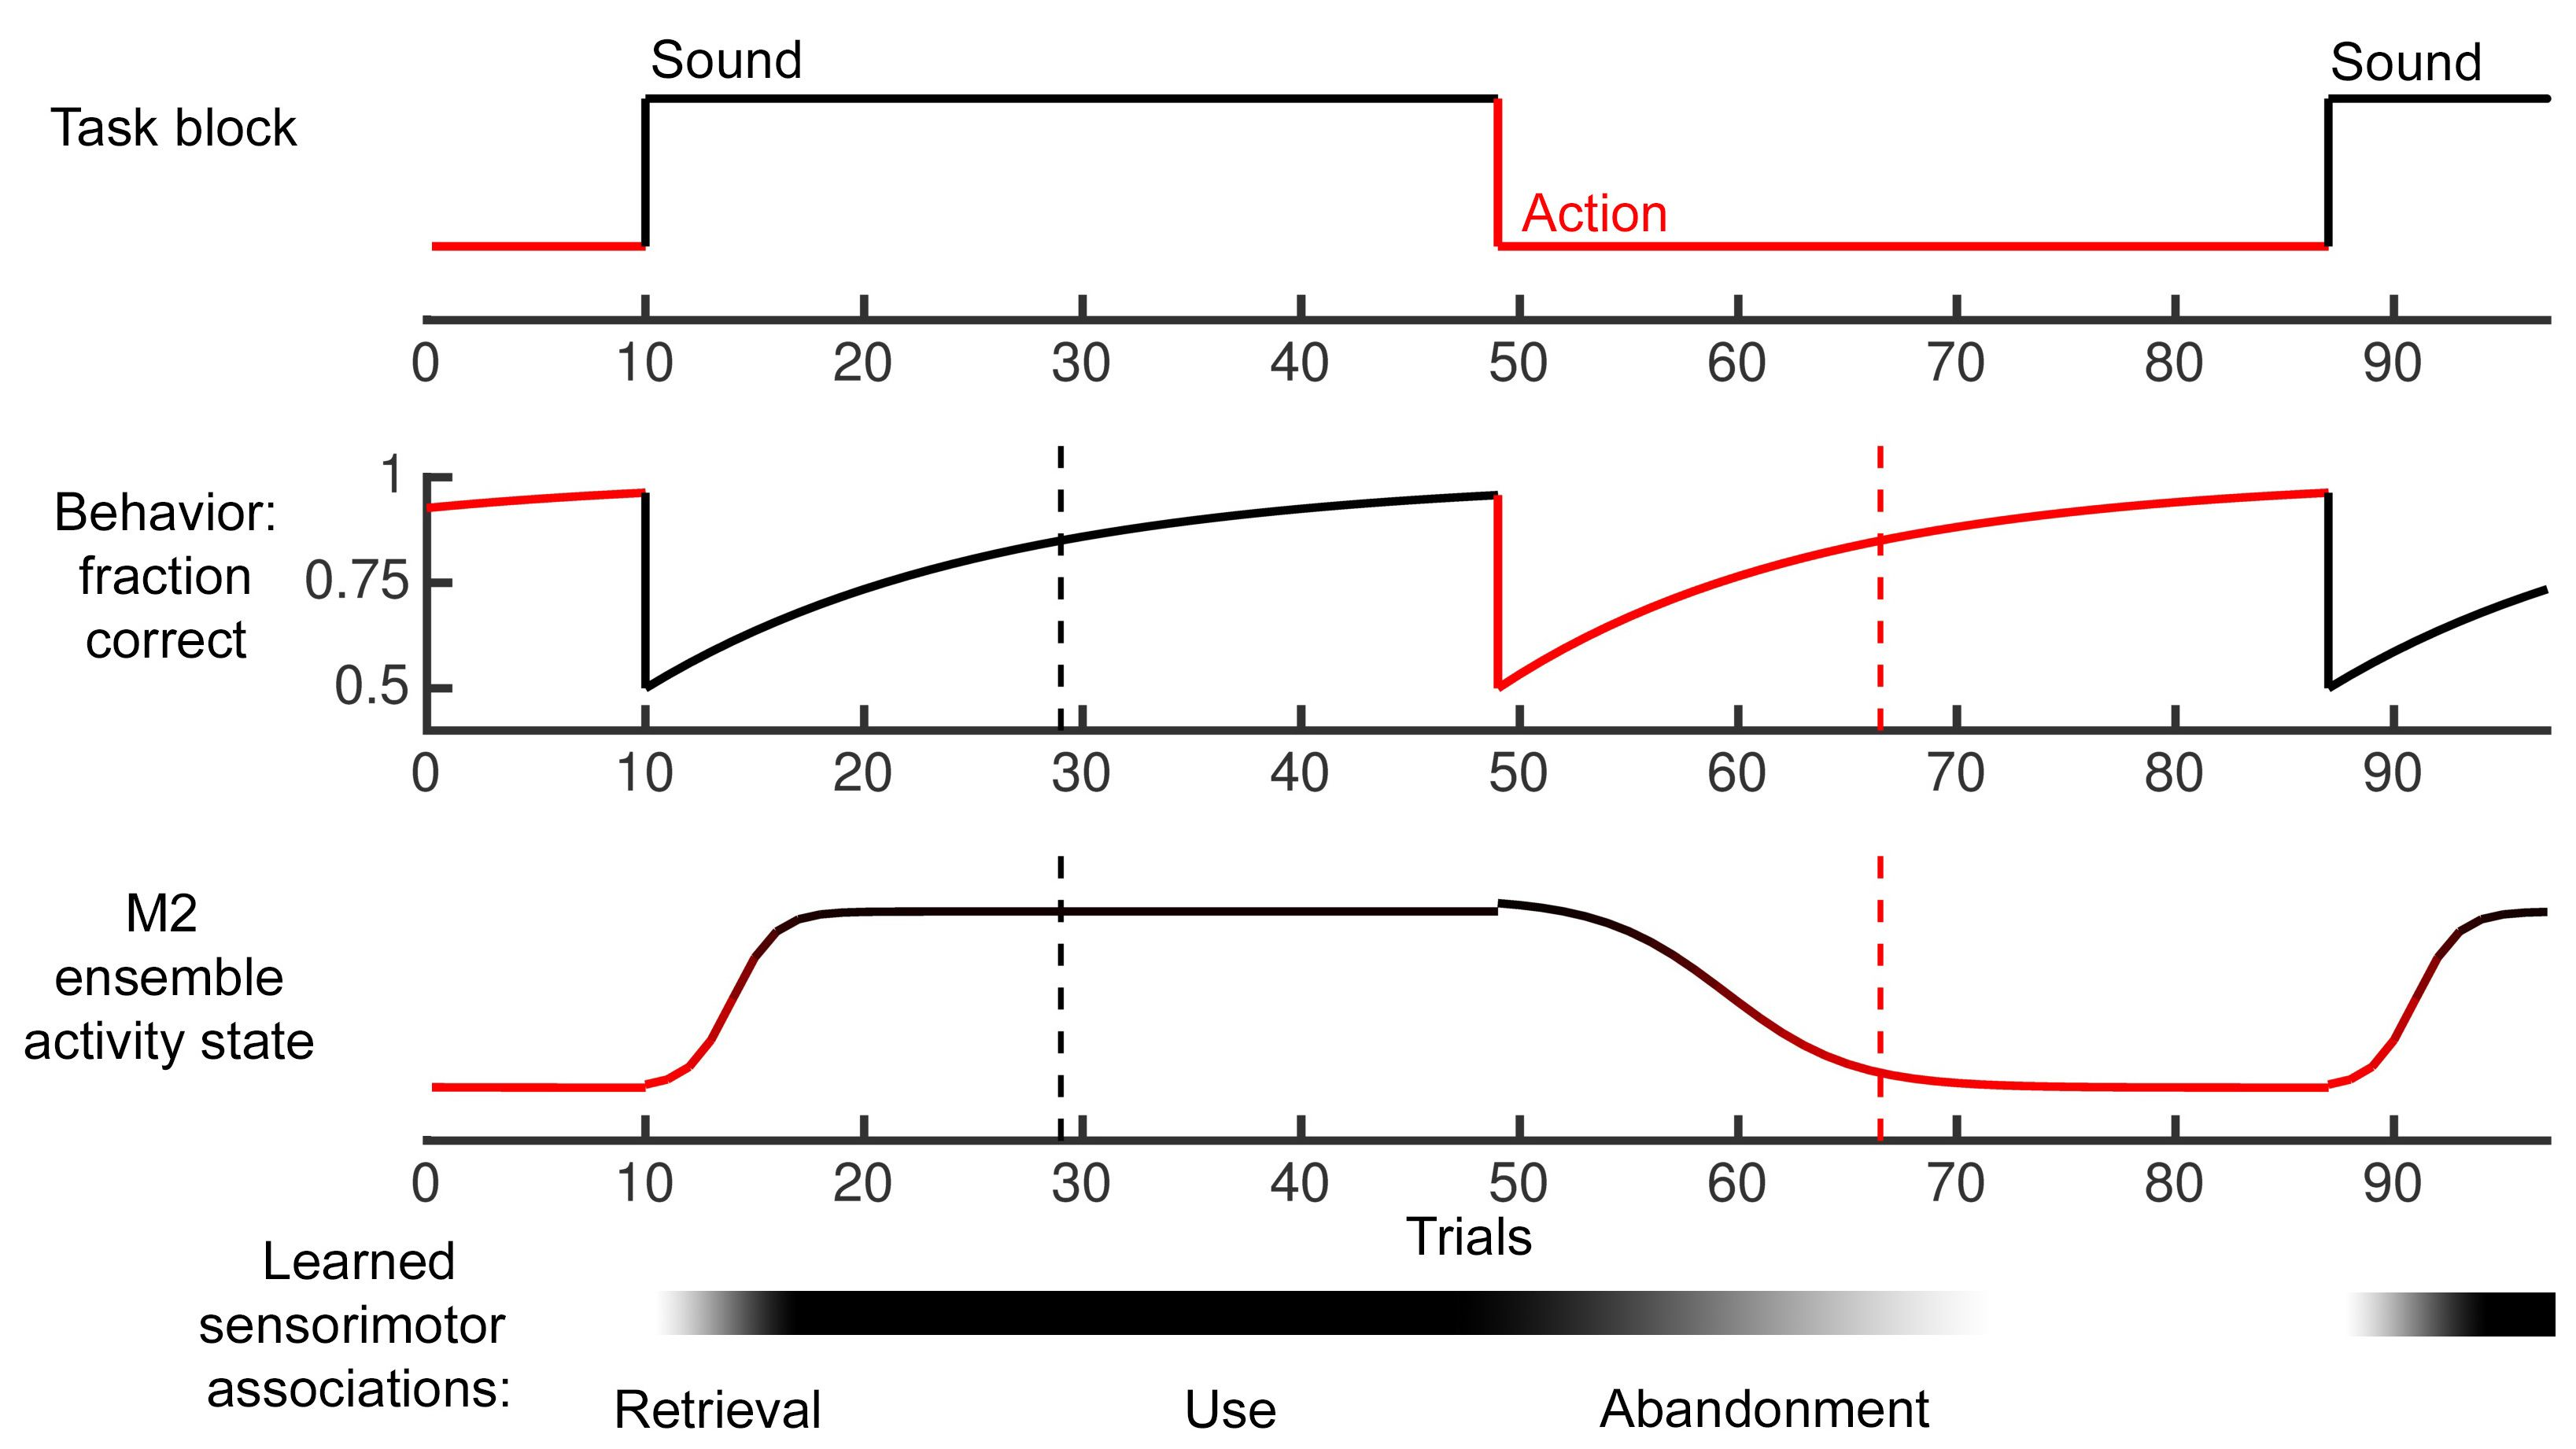
\includegraphics[width=\textwidth]{Figures/Chapter3/NN_figS9.jpg} 
\end{center}

\caption[Summary of the task, behavioral performance, and neural dynamics]
{Summary of the task, behavioral performance, and neural dynamics. (Top) Time course of experimentally imposed rule contingencies for a typical sound block, followed by a typical action block. (Middle) Recovery of behavioral performance following each rule switch was approximated as an exponential function for this schematic. Dashed lines reflect the median transition trial (sound: 19.0, action: 17.5). (Bottom) Same as \emph{middle} for the evolution of M2 ensemble activity relative to each rule switch (median transition trial---sound: 5.1, action: 14.6). State values are based on the midpoint trial (sound: 4.0, action: 10.4), steepness (sound: 1.02, action: 0.35), and range (sound: 0.36, action: 0.38) parameters estimated from logistic fits of the neural transition data (see Fig. \ref{fig:NN_fig4}).
}

\label{fig:NN_figS9}
\end{figure}